\begin{frame}
	\frametitle{Initialization}
	\begin{tikzpicture}[
	expl/.style={draw=black, thick=2pt,fill=blue!20,rounded corners},
	arrow/.style={red!80!black,ultra thick,->,>=latex}]	
	\node[anchor=south west,inner sep=0] (image) at (0,0) {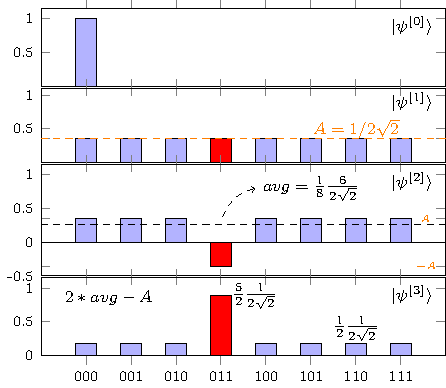
\includegraphics[width=0.5\textwidth]{figures/bar-graph/probs.pdf}};
	\begin{scope}[x={(image.south east)},y={(image.north west)}]
	%\draw[help lines,xstep=.1,ystep=.1] (0,0) grid (1,1);
	%\foreach \x in {0,1,...,9} { \node [anchor=north] at (\x/10,0) {0.\x}; }
	%\foreach \y in {0,1,...,9} { \node [anchor=east] at (0,\y/10) {0.\y}; }
	\node[expl](A) at (1.5,0.875) {\Large Initial state $\ket{\psi^{[0]}}$};
	\node[expl](B) at (1.5,0.65) {\Large Initialization $\ket{\psi^{[1]}}$};
	\node[expl](C) at (1.5,0.4) {\Large Sign flip $\ket{\psi^{[2]}}$};
	\node[expl](D) at (1.5,0.15) {\Large Inversion about average $\ket{\psi^{[3]}}$};
	
	\draw[arrow] (A.south) -- node [right]{Hadamard $H$} (B.north);
	\draw[arrow] (B.south) -- node [right]{Oracle $U_f$} (C.north);
	\draw[arrow] (C.south) -- node [right]{Difussion $U_d$} (D.north);
	\draw[thick,dashed] (0.01,0.575) rectangle (1.85,1);
	\draw[arrow] (D.north east) to[bend right] node [right]{$\frac{\pi}{4}\sqrt{n}$} (B.east);
	\end{scope}
	
	\end{tikzpicture}	
\end{frame}
\begin{frame}
\frametitle{Initialization}
We find a method (unitary operator) to have all the states with the same probability (\textit{principle of superposition}). 
\pause
\begin{eqnarray}
(I^{\otimes n}\otimes X)\left.|0\right\rangle _{n+1}&=&\left.|0\right\rangle _{n}\otimes\left.|1\right\rangle \nonumber\\
H^{\otimes\left(n+1\right)}\left[(I^{\otimes n}\otimes X)\left.|0\right\rangle _{n+1}\right]&=&H^{\otimes n}\left.|0\right\rangle _{n}\otimes H\left.|1\right\rangle \nonumber\\
&=&\sum_{j\in\{0,1\}^{n}}\frac{1}{\sqrt{2^{n}}}\left.|j\right\rangle _{n}\otimes\frac{1}{\sqrt{2}}\left(\left.|0\right\rangle -\left.|1\right\rangle \right)\nonumber\\
&=&\sum_{j\in\{0,1\}^{n}}\alpha_{j}\left.|j\right\rangle _{n}\otimes\frac{1}{\sqrt{2}}\left(\left.|0\right\rangle -\left.|1\right\rangle \right)\nonumber\\
&=&\ket{\psi^{[1]}}\nonumber
\end{eqnarray}
\end{frame}

\begin{frame}
\frametitle{Initialization}

\begin{exampleblock}{3-qubit example: Set ancillary qubit to $\ket{1}$}
\begin{eqnarray}
(I^{\otimes3}\otimes X)\left.|0\right\rangle _{3+1}&=&I^{\otimes3}\left.|0\right\rangle _{3}\otimes X\left.|0\right\rangle \nonumber\\
&=&\begin{pmatrix*}[c]
1&0&0&0&0&0&0&0\\
0&1&0&0&0&0&0&0\\
0&0&1&0&0&0&0&0\\
0&0&0&1&0&0&0&0\\
0&0&0&0&1&0&0&0\\
0&0&0&0&0&1&0&0\\
0&0&0&0&0&0&1&0\\
0&0&0&0&0&0&0&1\\
\end{pmatrix*}\left(\begin{array}{c}
1\\
0\\
0\\
0\\
0\\
0\\
0\\
0
\end{array}\right)\otimes\left(\begin{array}{cc}
0 & 1\\
1 & 0
\end{array}\right)\left(\begin{array}{c}
1\\
0
\end{array}\right)\nonumber\\
&=&\left.|0\right\rangle_3 \otimes\left.|1\right\rangle \nonumber
\end{eqnarray}
\end{exampleblock}


\end{frame}

\begin{frame}
\frametitle{Initialization}
\begin{exampleblock}{3-qubit example: Apply Hadamard gate}
\begin{eqnarray}
\ket{\psi^{[1]}}&=&H^{\otimes\left(3+1\right)}\left[(I^{\otimes3}\otimes X)\left.|0\right\rangle _{n+1}\right]\nonumber\\
&=&H^{\otimes3}\left.|0\right\rangle_3 \otimes H\left.|1\right\rangle\nonumber\\
&=&\frac{1}{\sqrt{2^{3}}}\begin{pmatrix*}[r]
1 & 1 & 1 & 1 & 1 & 1 & 1 & 1\\
1 & -1 & 1 & -1 & 1 & -1 & 1 & -1\\
1 & 1 & -1 & -1 & 1 & 1 & -1 & -1\\
1 & -1 & -1 & 1 & 1 & -1 & -1 & 1\\
1 & 1 & 1 & 1 & -1 & -1 & -1 & -1\\
1 & -1 & 1 & -1 & -1 & 1 & -1 & 1\\
1 & 1 & -1 & -1 & -1 & -1 & 1 & 1\\
1 & -1 & -1 & 1 & -1 & 1 & 1 & -1
\end{pmatrix*}\left(\begin{array}{c}
1\\
0\\
0\\
0\\
0\\
0\\
0\\
0
\end{array}\right)\otimes\frac{1}{\sqrt{2}}\left(\begin{array}{cc}
1 & 1\\
1 & -1
\end{array}\right)\left(\begin{array}{c}
0\\
1
\end{array}\right)\nonumber
\end{eqnarray}
\end{exampleblock}
\end{frame}

\begin{frame}
	\frametitle{Initialization}
	\begin{exampleblock}{3-qubit example: Apply Hadamard gate}
		\begin{eqnarray}
			\ket{\psi^{[1]} }&=&\frac{1}{\sqrt{2^{3}}}\begin{pmatrix*}
			1 1 1 1 1 1 1 1
			\end{pmatrix*}^{\dagger}\otimes\frac{1}{\sqrt{2}}\left(\begin{array}{c}
			1\\
			-1
			\end{array}\right)\nonumber\\
			&=&[ \frac{1}{2\sqrt{2}}\left.|000\right\rangle +\frac{1}{2\sqrt{2}}\left.|001\right\rangle +\frac{1}{2\sqrt{2}}\left.|010\right\rangle +\frac{1}{2\sqrt{2}}\left.|011\right\rangle \nonumber\\
			&+&\frac{1}{2\sqrt{2}}\left.|100\right\rangle +\frac{1}{2\sqrt{2}}\left.|101\right\rangle +\frac{1}{2\sqrt{2}}\left.|110\right\rangle +\frac{1}{2\sqrt{2}}\left.|111\right\rangle] \nonumber\\
			&\otimes&\frac{1}{\sqrt{2}}\left(\left.|0\right\rangle -\left.|1\right\rangle \right)		\nonumber	
		\end{eqnarray}
	\end{exampleblock}
\end{frame}

\begin{frame}{}
	\frametitle{Initialization}
	\begin{exampleblock}{3-qubit example: Summary}
		\begin{eqnarray}
			\ket{\psi^{[1]} }&=&
			H^{\otimes\left(3+1\right)}\left[(I^{\otimes3}\otimes X)\left.|0\right\rangle _{n+1}\right]\nonumber\\
			&=&[\frac{1}{2\sqrt{2}}\left.|000\right\rangle +\frac{1}{2\sqrt{2}}\left.|001\right\rangle +\frac{1}{2\sqrt{2}}\left.|010\right\rangle +\frac{1}{2\sqrt{2}}\left.|011\right\rangle\nonumber\\ &+&\frac{1}{2\sqrt{2}}\left.|100\right\rangle +\frac{1}{2\sqrt{2}}\left.|101\right\rangle +\frac{1}{2\sqrt{2}}\left.|110\right\rangle +\frac{1}{2\sqrt{2}}\left.|111\right\rangle ]\nonumber\\
			&\otimes&\frac{1}{\sqrt{2}}\left(\left.|0\right\rangle -\left.|1\right\rangle \right)\nonumber\\
			&=&\sum_{j\in\{0,1\}^{n}}\frac{1}{\sqrt{2^{n}}}\left.|j\right\rangle _{n}\otimes\frac{1}{\sqrt{2}}\left(\left.|0\right\rangle -\left.|1\right\rangle \right)=\ket{\psi^{[1]} }\nonumber
		\end{eqnarray}
	\end{exampleblock}
\end{frame}


